\section*{Part 3 [68 points]}

\begin{enumerate}
    \item \textbf{[34 points]} Describe and analyze your hand-crafted policy. 
    \begin{enumerate}
    \item \textbf{[17 points]} With your scheduling policy, run the entire workflow \textbf{\textcolor{red}{3 separate times}}. For each run, measure the execution time of each batch job, as well as the latency outputs of memcached, running with a steady client load of 30K QPS. For each batch application, compute the mean and standard deviation of the execution time \footnote{Here, you should only consider the runtime, excluding time spans during which the container is paused.} across three runs. Also, compute the mean and standard deviation of the total time to complete all jobs - the makespan of all jobs. Fill in the table below. Finally, compute the SLO violation ratio for memcached for the three runs; the number of data points with 95th percentile latency $>$ 1ms, as a fraction of the total number of data points. The SLO violation ratio should be calculated during the time from when the first batch-job-container starts running to when the last batch-job-container stops running.  \\

    \begin{table}[ht]
        \centering
        \begin{tabular}{ |c|c|c|c|c|} 
            \hline
            job name & mean time [s] & std [s] \\ \hline \hline
            \coloredcell{barnes}          & 23.67 & 0.58 \\  \hline
            \coloredcell{blackscholes}    & 110.00 & 4.36 \\  \hline
            \coloredcell{canneal}         & 139.33 & 7.23 \\  \hline
            \coloredcell{freqmine}        & 68.33 & 0.58 \\  \hline
            \coloredcell{radix}           & 6.00 & 0.00 \\  \hline
            \coloredcell{streamcluster}   & 105.00 & 4.58 \\  \hline
            \coloredcell{vips}            & 74.00 & 8.54 \\  \hline
            total time      & 219.67 & 10.79 \\  \hline
        \end{tabular}
    \end{table}

    \textbf{Answer:} % Place your solution here.

    The displayed results are averaged over 3 seperate runs.

    The execution time for the individual jobs is relatively stable with minor differences between the runs of longer running jobs.

    The execution time for all jobs in total is on average $219.67$ seconds with a larger standard deviation of $10.79$ seconds. This relates to the difference in the execution times of the longer running.

    With our policy, there are 0 datapoints with 95th percentile latency $> 1ms$. Therefore, our SLO violation ration is $0\%$.

    \[\text{SLO violaition ration} = \frac{\text{\#datapoints with p95} > 1 \text{ms}}{\text{\#p95 datapoints}} = \frac{0}{\text{\#p95 datapoints}} =  0\%\]
        
    

    
    Create 3 bar plots (one for each run) of memcached p95 latency (y-axis) over time (x-axis), with annotations showing when each batch job started and ended, also indicating the machine each of them is running on. Using the augmented version of mcperf, you get two additional columns in the output: \texttt{ts\_start} and \texttt{ts\_end}. Use them to determine the width of each bar in the bar plot, while the height should represent the p95 latency. Align the $x$ axis so that $x=0$ coincides with the starting time of the first container. 
    For each core in each machine show what job it is running using the colors proposed in this template (you can find them in \texttt{main.tex}). For example, draw a bar in {\color{vips}the color of vips} for core x from when vips is started to when it ends if vips ran on core x.
    %Use  the colors proposed in this template (you can find them in \texttt{main.tex}). For example, use the \colored{vips} color to annotate when vips started and stopped, the \colored{blackscholes} color to annotate when blackscholes started and stopped etc.

    \textbf{Plots:} % Place your plots here.
    \begin{figure}[H]
        \centering
        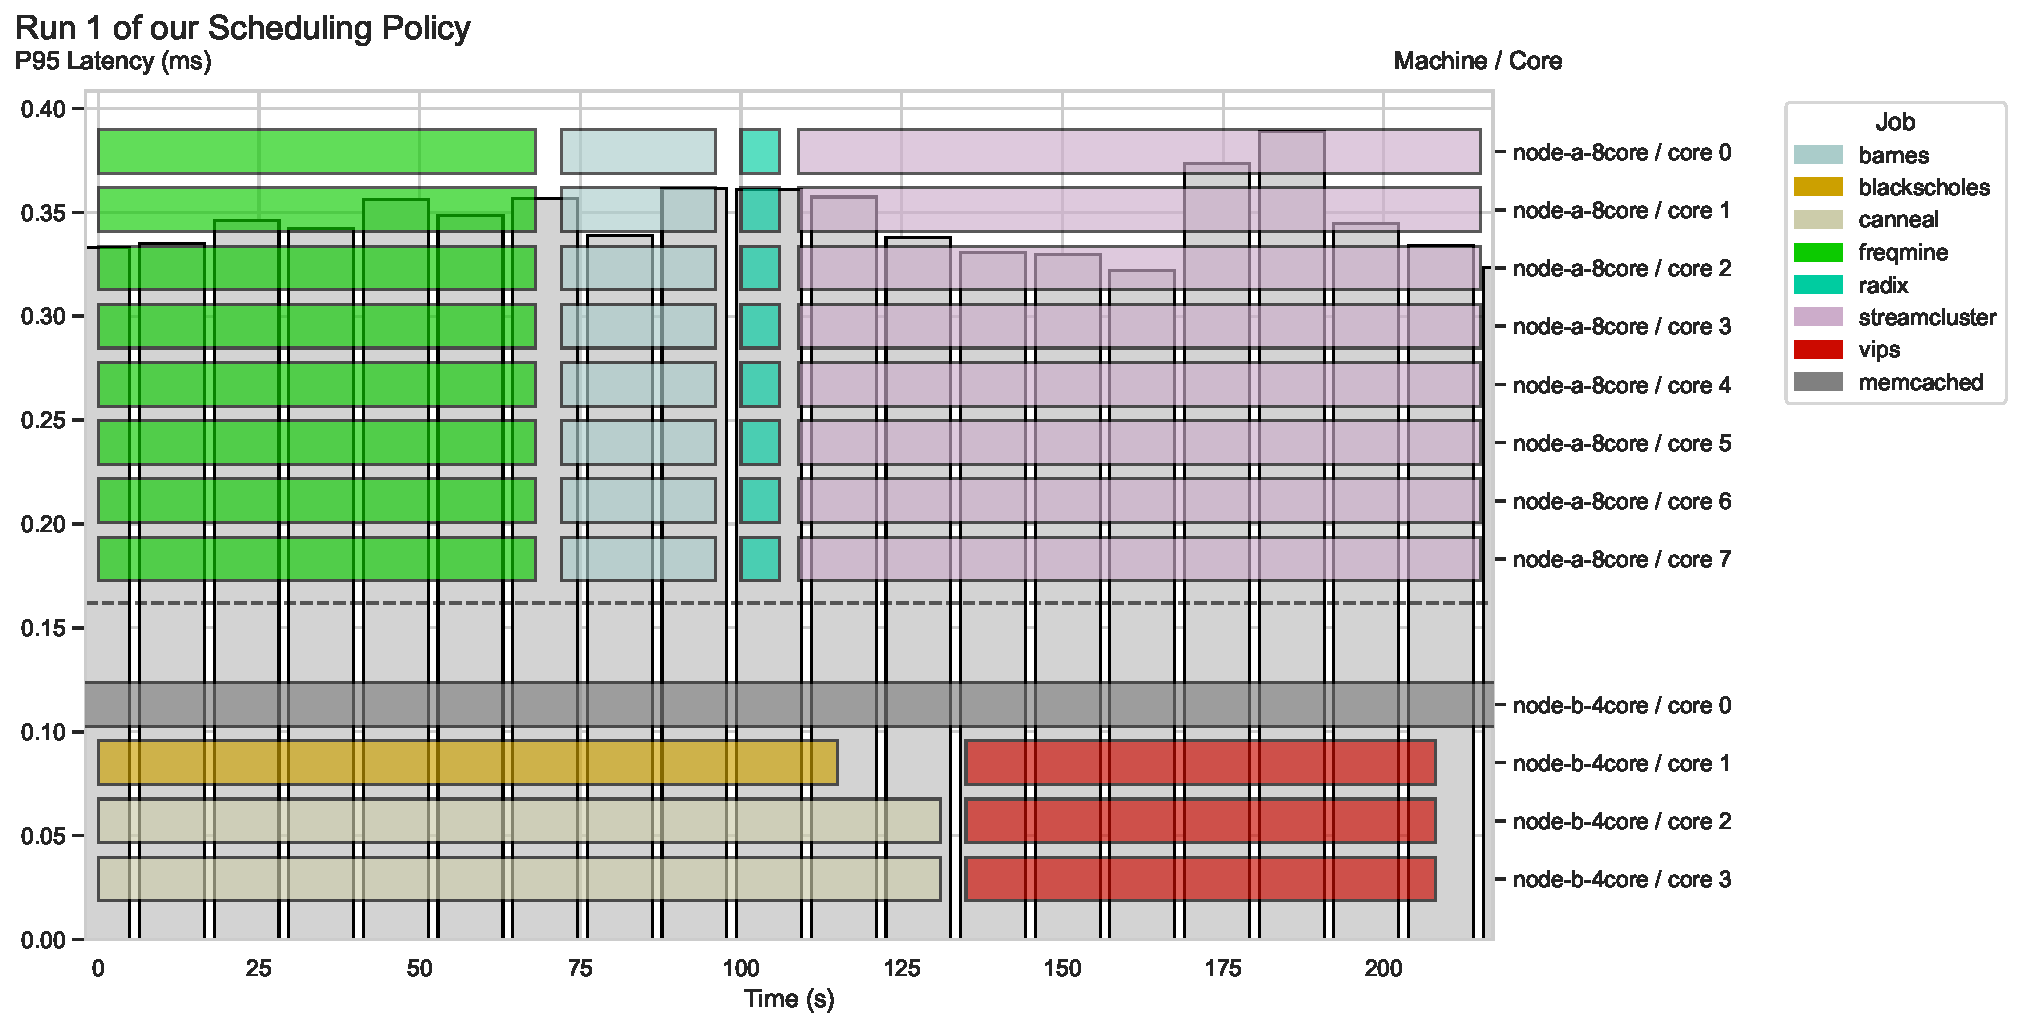
\includegraphics[width=1\linewidth]{report/figures/part3_0.pdf}
        \caption{First run of our policy, having the shortest run time of all runs with 212 seconds. Showing the running time in seconds on the x-axis, the 95th percentile latency of memcached on the left y-axis, represented by gray vertical bars in the background), and on the right y-axis the nodes and its cores, where a color-coded vertical bar shows which job is running on that specific core. The 95th percentile latency constantly stayed below $0.4 ms$, meeting the SLO of $1ms$.}
        \label{fig:part3_0}
    \end{figure}

    \begin{figure}[H]
        \centering
        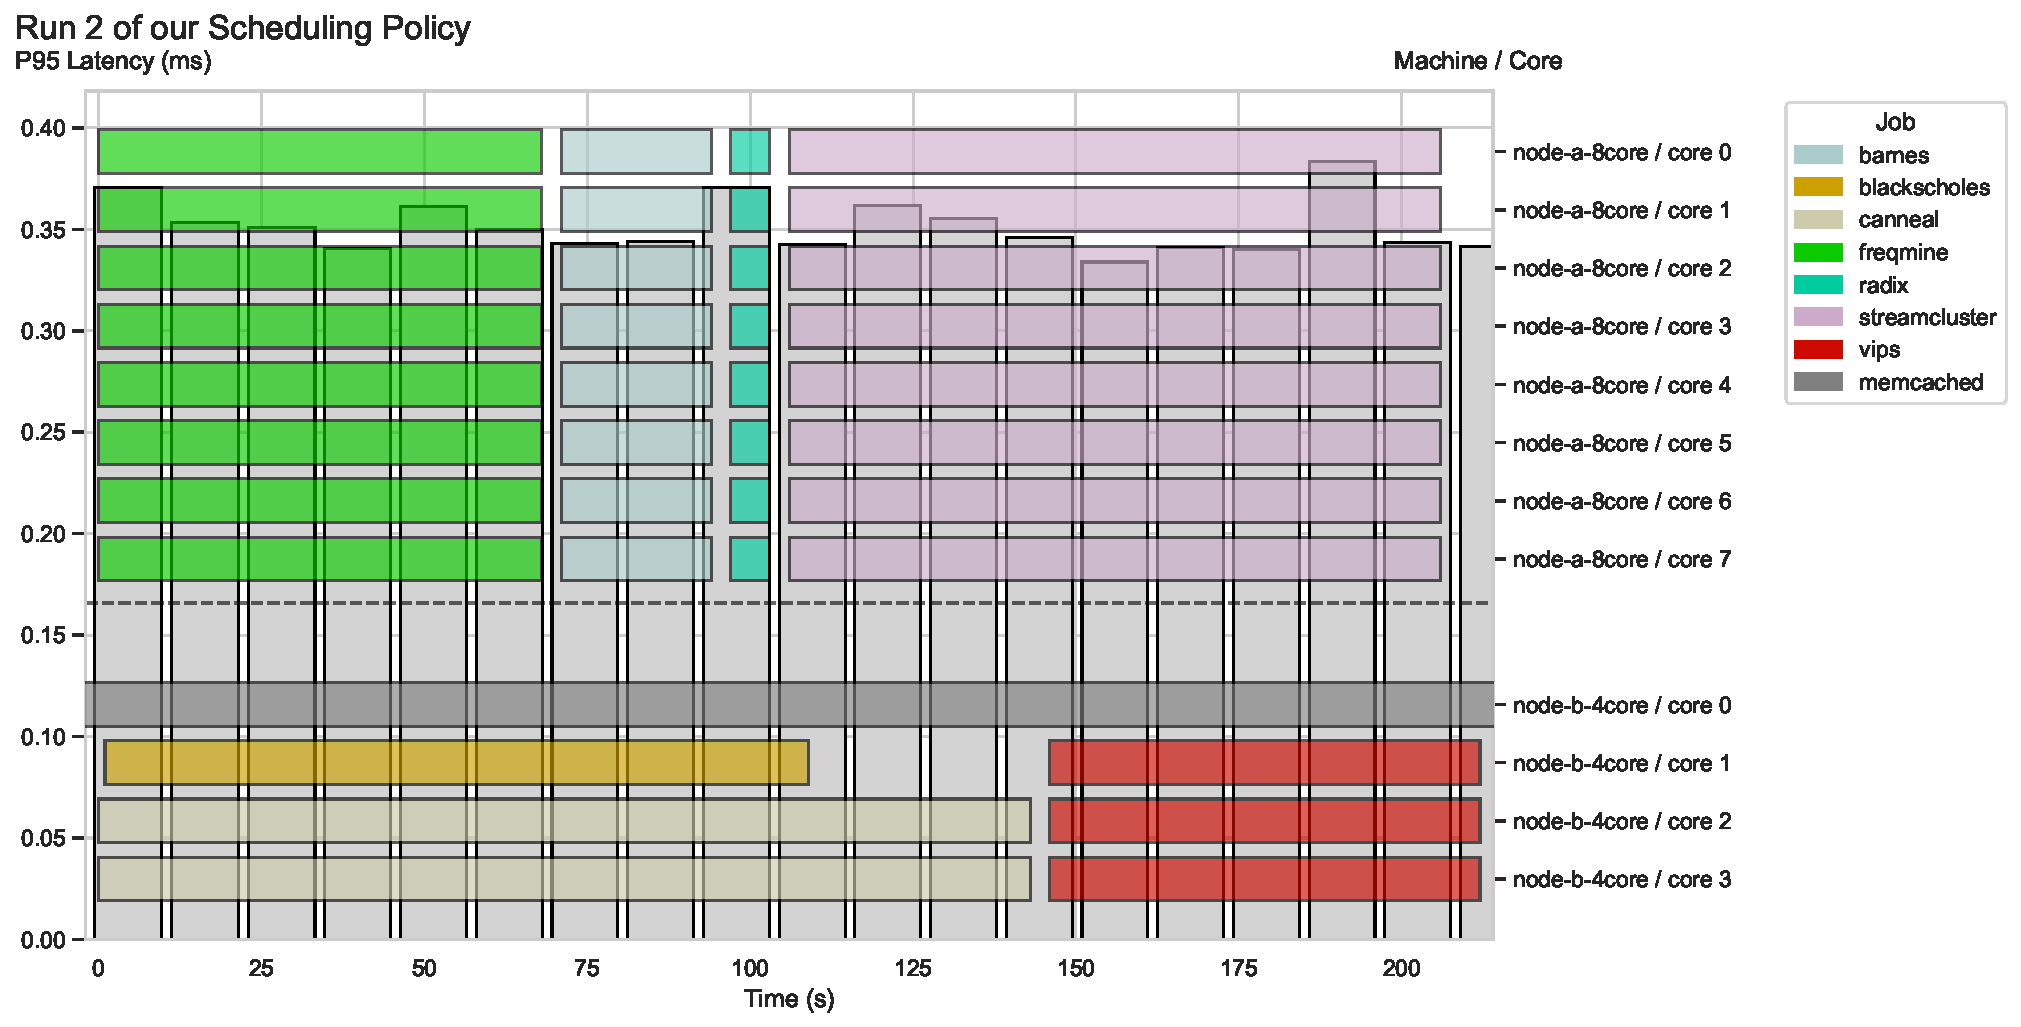
\includegraphics[width=1\linewidth]{report/figures/part3_1.pdf}
        \caption{Second run of our policy, having a run time of 215 seconds. Showing the running time in seconds on the x-axis, the 95th percentile latency of memcached on the left y-axis, represented by gray vertical bars in the background), and on the right y-axis the nodes and its cores, where a color-coded vertical bar shows which job is running on that specific core. The 95th percentile latency constantly stayed below $0.4 ms$.}
        \label{fig:part3_1}
    \end{figure}

    \begin{figure}[H]
        \centering
        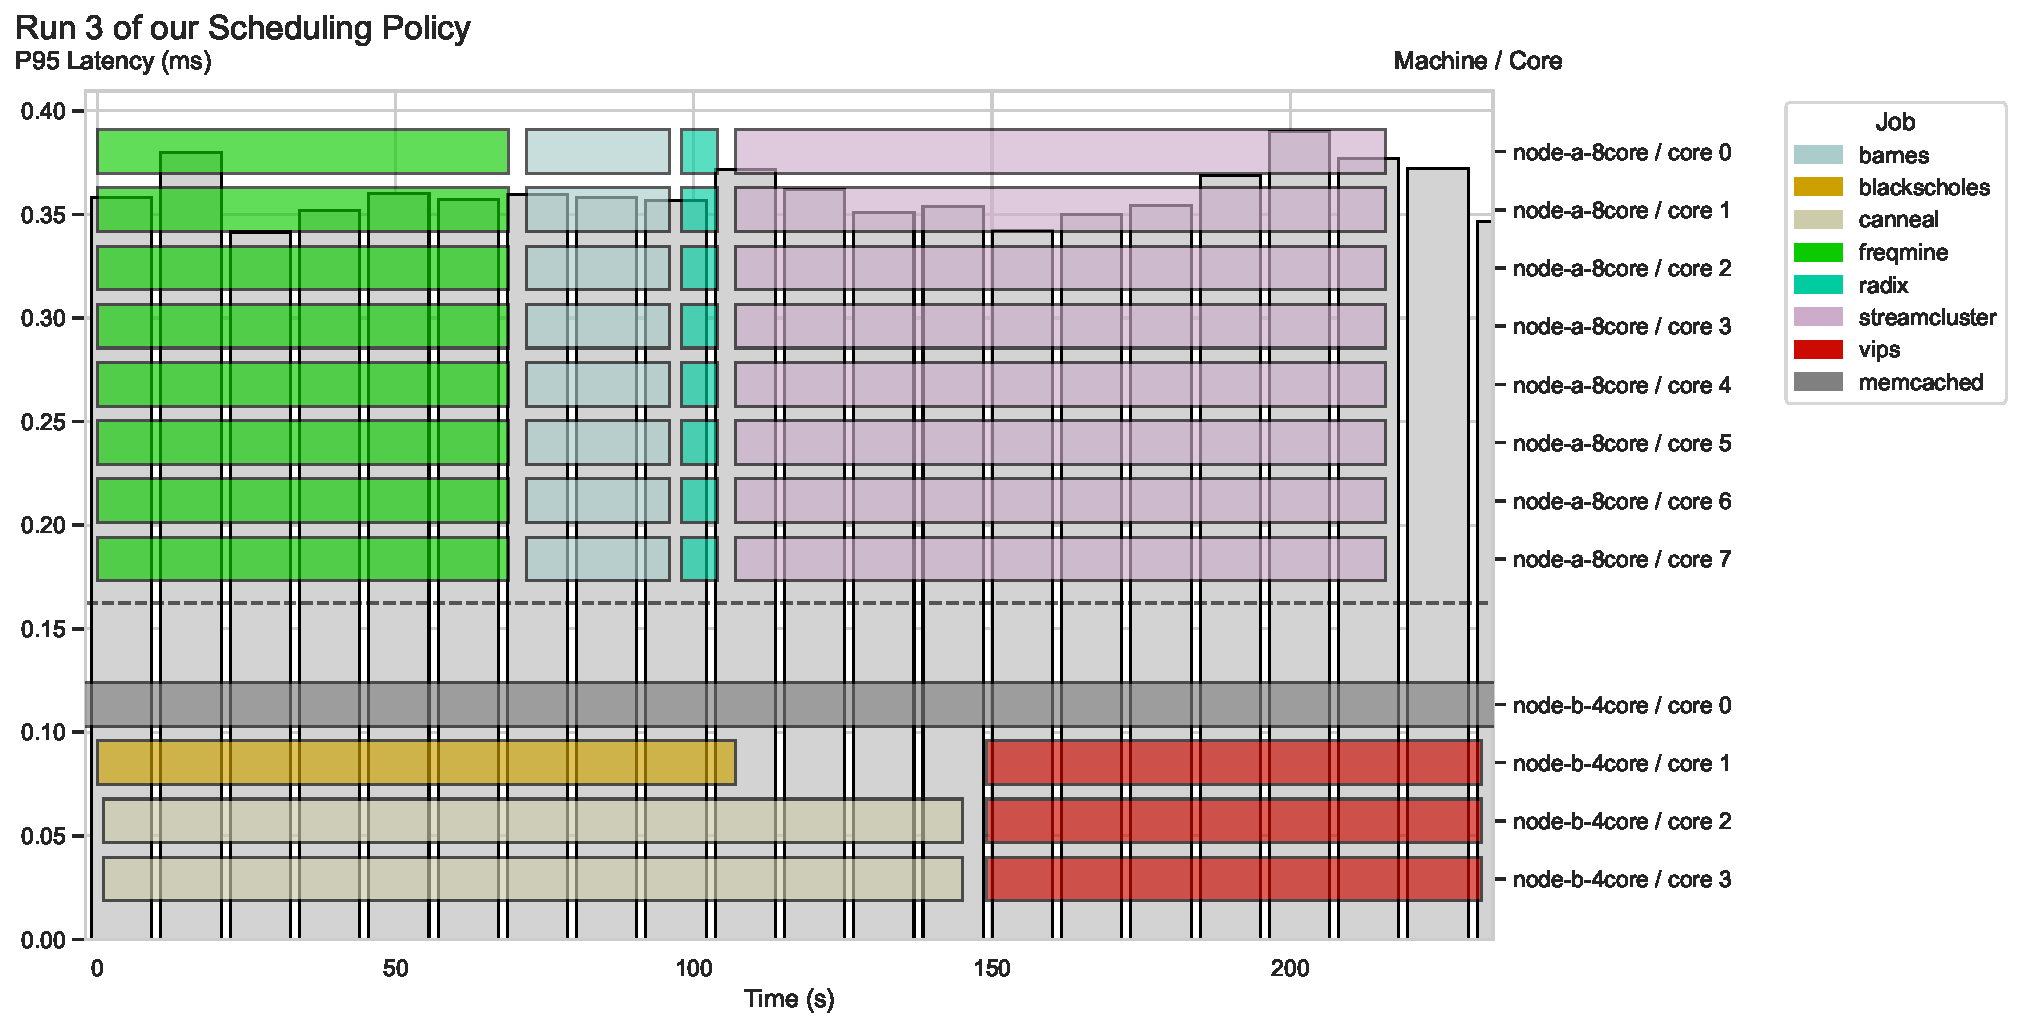
\includegraphics[width=1\linewidth]{report/figures/part3_2.pdf}
        \caption{Third run of our policy, having a run time of 232 seconds. Showing the running time in seconds on the x-axis, the 95th percentile latency of memcached on the left y-axis, represented by gray vertical bars in the background), and on the right y-axis the nodes and its cores, where a color-coded vertical bar shows which job is running on that specific core. The 95th percentile latency constantly stayed below $0.4 ms$.}
        \label{fig:part3_2}
    \end{figure}
        
    \item \textbf{[17 points]} Describe and justify the “optimal” scheduling policy you have designed. 
    
    \begin{itemize}
        \item Which node does memcached run on? Why?

        \textbf{Answer:} memcached runs on node-b-4core, as this node has a better performance than the other node.
        \\

        \item Which node does each of the 7 batch jobs run on? Why?

        \textbf{Answer:}
        \begin{itemize}
            \item \colored{barnes}: Barnes runs on node-a-8core, as in Part 2 there was a significant speedup observable when increasing the number of threads for this job.
            
            \item \colored{blackscholes}: Blackscholes runs on node-b-4core, as it did not show large interference effects on resources where memcached was showing high effects, suggesting that collocating both on the same node will not increase the 95th percentile latency. Additionally, this job did not scale very well when increasing the number of threads, which also can only happen in powers of two, so it is run on the node with the better performance.
            
            \item \colored{canneal}: Blackscholes runs on node-b-4core, as it did not show large interference effects on resources where memcached was showing high effects, suggesting that collocating both on the same node will not increase the 95th percentile latency. Additionally, this job did not scale very well when increasing the number of threads, which also can only happen in powers of two, so it is run on the node with the better performance.
            
            \item \colored{freqmine}: Freqmine runs on node-a-8core, as in Part 2 there was a significant speedup observable when increasing the number of threads for this job.
            
            \item \colored{radix}: Radix runs on node-a-8core, as in Part 2 there was a significant speedup observable when increasing the number of threads for this job.
            
            \item \colored{streamcluster}:Streamcluster runs on node-a-8core, as in Part 2 there was a significant speedup observable when increasing the number of threads for this job.
            
            \item \colored{vips}: Vips runs on node-b-4core, as it only showed medium interference effects on resources where memcached was showing high effects, suggesting that collocating both on the same node will not increase the 95th percentile latency. Additionally, this job did not scale very well when increasing the number of threads, which also can only happen in powers of two, so it is run on the node with the better performance.
            \\
            
        \end{itemize}

        \item Which jobs run concurrently / are colocated? Why?

        \textbf{Answer:} Memcached is running non-stop on node-b-4core, thus beeing collocated with the other jobs running on this core (blackscholes, canneal, and vips). All of the mentioned jobs have shown only little or medium interference effects on resources affecting memcached the most and therefore it can be assumed that they do not increase the 95th percentile latency of memcached.

        Additionally, blackscholes and canneal are collocated on node-b-4core, as both of them have relatively low interference effects, and where blackscholes had medium interference with l2 cache, canneal has small interference effects. As they run on different cores, cpu and level 1 caches are isolated and do not interfere.
        \\

        \item In which order did you run the 7 batch jobs? Why?
    
        \textbf{Order (to be sorted)}:
        
        node-a-8core: \colored{freqmine}, \colored{barnes}, \colored{radix}, \colored{streamcluster}
        
        node-b-4core: $\{$\colored{blackscholes}, \colored{canneal}$\}$, \colored{vips}
    
    
        \textbf{Why}: % Place your solution here.
        There was no particular reason to start the jobs in the mentioned order for the node-a-8core, as they all run on all 8 cores and therefore are executed sequentially.

        For the node-b-4core, first the two jobs that run in parallel were started at the same time (blackscholes and canneal), as the duration of both jobs, in the way there are scheduled here, is very similar and they finish at a very similar time. Afterwards, the vips job i scheduled. Again, there was no paticular reason that first the blackscholes and canneal and then vips is scheduled, as they are supposed to run sequentially.
        \\

        \item How many threads have you used for each of the 7 batch jobs? Why?
    
        \textbf{Answer:}
    
        \begin{itemize}
            \item \colored{barnes}: 8 threads, as it showed speedup gain in Part 2 when running it on 8 threads, and as this is a SPLASH-job, the number of threads should be a power of 2. 
            
            \item \colored{blackscholes}: 1 thread, as it did not show a high speedup in Part 2, and when it is run on one thread it finishes at a similar time as canneal run on 2 threads (shorter total runtime).
            
            \item \colored{canneal}: 2 threads, as it only showed a limited speedup in Part 2 when increasing the number of threads, and it takes a similar time to finish when being run on 2 threads as blackscholes being run on 1 thread.
            
            \item \colored{freqmine}: 8 threads, as it showed significant speedup in Part 2 when running it on 8 threads.
            
            \item \colored{radix}: 8 threads, as it showed significant, almost linear speedup in Part 2 when running it on 8 threads, and as this is a SPLASH-job, the number of threads should be a power of 2.
           
            \item \colored{streamcluster}: 8 threads, as it showed significant speedup in Part 2 when running it on 8 threads.
            
            \item \colored{vips}: 3 threads, as it showed limited but slightly better speedup when increasing the number of threads, is the last task to be executed and therefore can receive the remaining threads, and finishes in a similar time as the tasks on on node-a-8core.
            \\
        \end{itemize}

        \item Which files did you modify or add and in what way? Which Kubernetes features did you use?
    
        \textbf{Answer:} % Place your solution here.
        TODO (andres): answer thorough process, files, concice but detailed.
        every file mention, what we did, supported process, and the reason why.
        \\ 
        
    
        \item Describe the design choices, ideas and trade-offs you took into account while creating your scheduler (\underline{if not already mentioned above}). Describe how your policy (and its performance) compares to another policy that you experimented with (in particular to the second-best policy that you designed).

        \textbf{Answer:} % Place your solution here
        The first design choice we took into account was the interference of memcached with resources and how well the jobs scale with different numbers of threads. Also, as the intereference for memcached for the CPU and the L1 cache was high, we decided to let it run isolated on one core of the node. We also took the same decision for all jobs, as most jobs were showing medium effects on interference with one of these components. We were also iterating over different setups and were checking on when memcached was violating the SLO of $1 ms$, e.g. when collocating canneal vips and barends together, and tried to avoid these situations in our scheduler. From previous runs we also observed the total runtime of different jobs and identified which jobs have a similar runtime and puzzled these jobs together in a way, that no node and CPU runs idle and both CPUs finish at a similar time. Additionally, we were taking into account that the nodes have a different performance. Therefore, we decided to let jobs that showed less effects when running it on multiple cores to be run on the more powerful machine, the node-b-4core. On the same machine we also decided to run memcached to give it compute-power to stay below the SLO.

        With our design choices we had to make multiple trade-offs. We decided to run most jobs in isolation, e.g., we ran all jobs on node-a-8core sequentially, therefore reduced the possibilities of parallelilsm of tasks, when being collocated on the same node. We took the same decision in regards of the cores, also reducing the possibilities for parallelism, as no jobs are collocated on the same core. Additionally, we decided to be careful with regards of the SLO, keeping the 95th percentile latency below $1 ms$, and therefore reduced the number of tasks running in parallel and therefore the overall runtime we could achieve.

        In our second best policy, next to memcached, only two jobs were running on the node-b-4core starting at the same time: canneal was running on one thread and blackscholes was running on two threads, according to their limited speedup when running on more cores. The blackscholes job was finished way earlier than the canneal job, and both jobs were finished earlier than the jobs running on the node-a-8core. This was leading to node-b-4core being being $\approx 25\%$ idle over the complete run. Therefore, we decided to give canneal two cores and blackscholes 1, so they finish at around the same time. The jobs freqmine, barnes, and radix were scheduled as in our final policy, running sequentially on node-a-8core. After they have finished, streamcluster and vips were scheduled at the same time, each running on 4 cores, as their achieved speedup in Part 2 was less than for the other jobs running on that node. This was also leading to the node being idle at the end. Thus, we decided to use the good scaling streamcluster was sowing for 8 cores in previous tasks, and let it run on all threads after the other ones were finsihed. We also decided to move vips to the 4core node, as it is a rather short job, that could fill the idle time of node-b-4core. In comparison to this policy, our final policy was stricter regarding collocation on node-a-8care, but already had the same isolation in regards to cores, as on each core always only one job was running. The 95th percentile latency was on average slightly higher in our old policy (slightly over $0.4 ms$) than in our final policy. It took over $100 s$ longer with $343 ms$ in our measured runs.
        \\
    
    \end{itemize}
    \end{enumerate}
    \item \textbf{[34 points]} Describe and analyze the AI-generated policy. [TODO: Xiaozhe]

    \begin{enumerate}
        \item \textbf{[17 points]} \textbf{Report the performance}:
        
        \begin{itemize}
            \item Report the mean time of each batch job, as well as the makespan of all jobs for the AI-generated policy. Also, report the SLO violation ratio for memcached for the AI-generated policy. \textit{Note: If the LLM failed to produce a valid solution after 3+ attempts, provide the error logs and your best-performing manual tweak for partial credit.}
        
        \begin{table}[ht]
            \centering
            \begin{tabular}{ |c|c|c|c|c|} 
                \hline
                job name & mean time [s] (Baseline) & mean time [s] (AI) \\ \hline \hline
                \coloredcell{barnes}          & 23.67 & 65.00 \\  \hline
                \coloredcell{blackscholes}    & 110.00 & 70.00 \\  \hline
                \coloredcell{canneal}         & 139.33 & 182.67 \\  \hline
                \coloredcell{freqmine}        & 68.33 & 192.33 \\  \hline
                \coloredcell{radix}           & 6.00 & 64.33 \\  \hline
                \coloredcell{streamcluster}   & 105.00 & 221.00 \\  \hline
                \coloredcell{vips}            & 74.00 & 37.67 \\  \hline
                total time      & 219.67 & 348.33 \\  \hline
            \end{tabular}
        \end{table}

    \item Create 3 bar plots (one for each run), for the final AI-generated policy, of memcached p95 latency (y-axis) over time (x-axis), with annotations showing when each batch job started and ended, also indicating the machine each of them is running on. Use the same method as described in the previous question to create the bar plots.
    
    \textbf{Answer:}

    \begin{figure}[H]
        \centering
        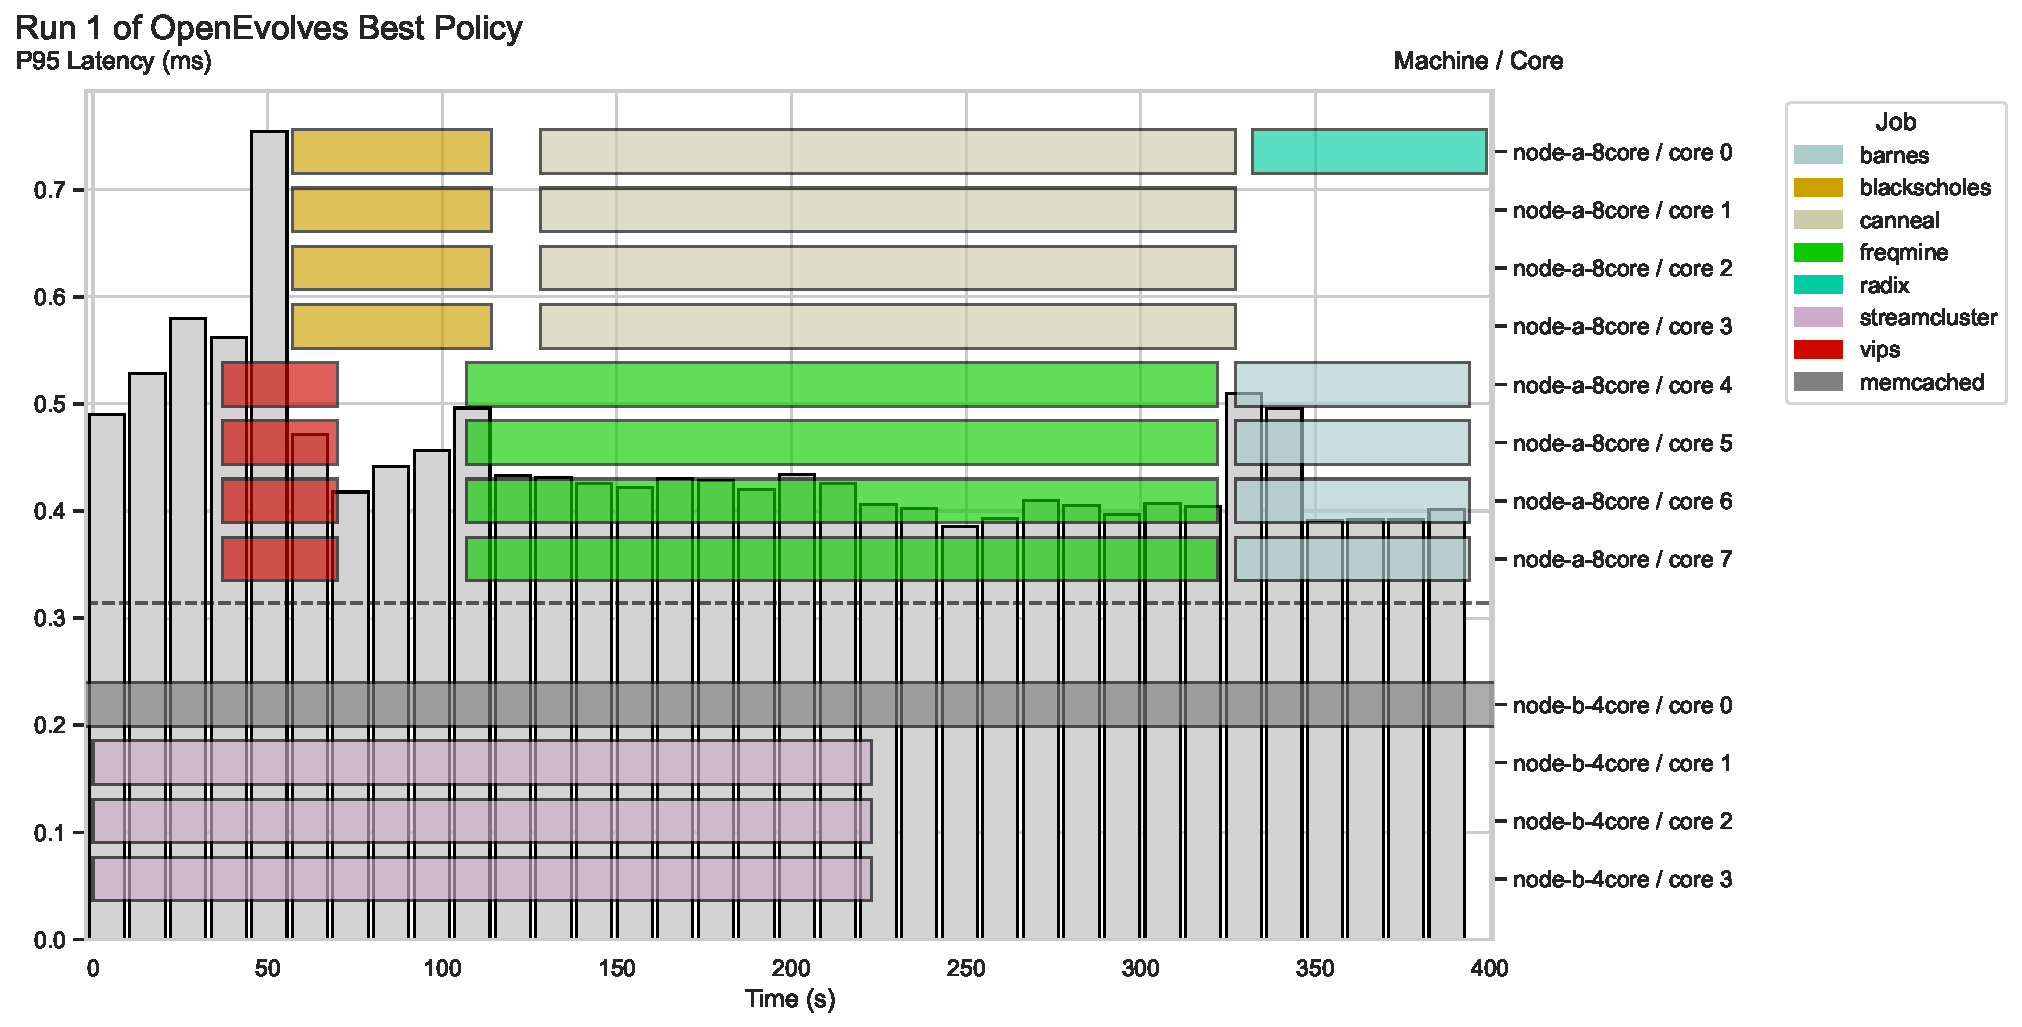
\includegraphics[width=1\linewidth]{report/figures/part3_2_0.pdf}
        \caption{First run of the AI-generated policy. Showing the running time in seconds on the x-axis, the 95th percentile latency of memcached on the left y-axis, represented by gray vertical bars in the background), and on the right y-axis the nodes and its cores, where a color-coded vertical bar shows which job is running on that specific core. The plot shows a larger startup delay for vips, blackscholes, and freqmine on the cloud, increasing the runtime, due to fetching the jobs in the first run. The 95th percentile latency mostly stayed below $0.6 ms$, despite one outlier reaching $0.75 ms$ but staying below the SLO of $1 ms$. The total time to finish all jobs was $399 s$.}
        \label{fig:part3_2_0}
    \end{figure}

    \begin{figure}[H]
        \centering
        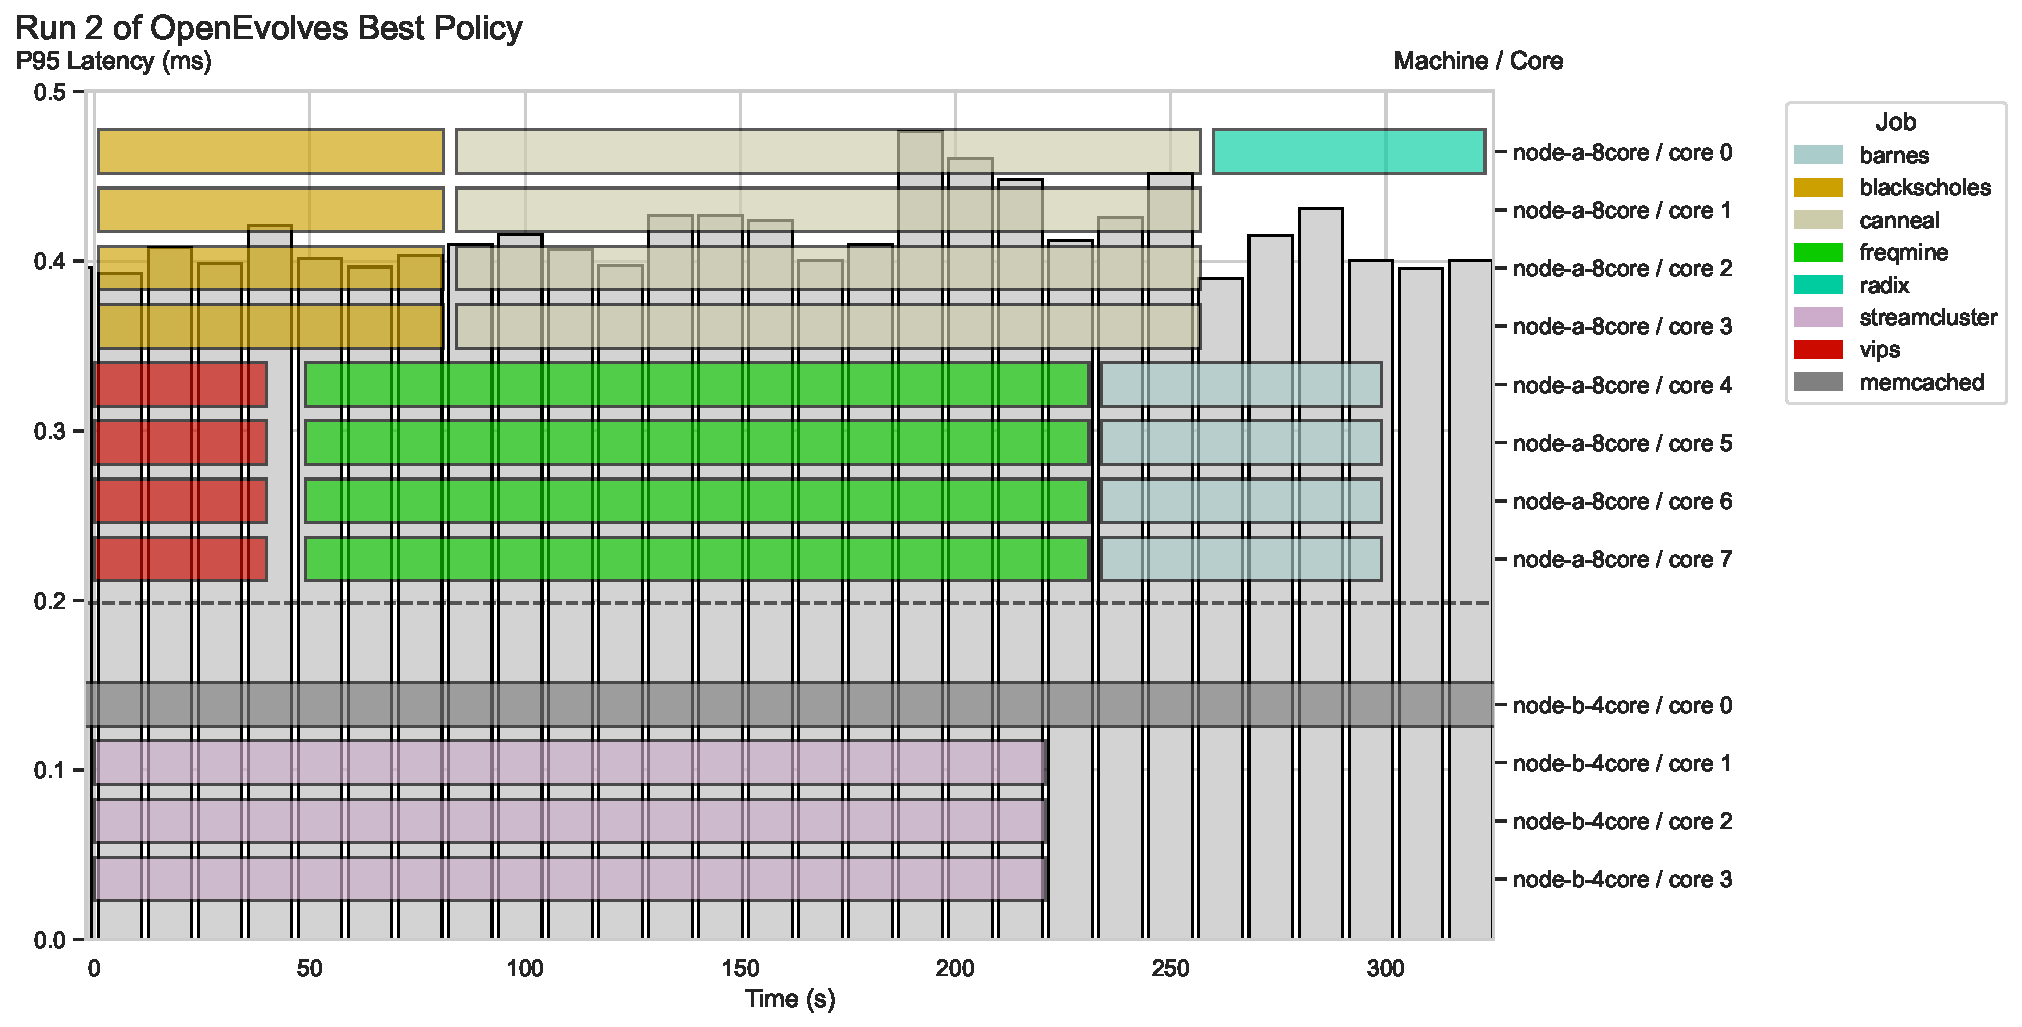
\includegraphics[width=1\linewidth]{report/figures/part3_2_1.pdf}
        \caption{Second run of the AI-generated policy. Showing the running time in seconds on the x-axis, the 95th percentile latency of memcached on the left y-axis, represented by gray vertical bars in the background), and on the right y-axis the nodes and its cores, where a color-coded vertical bar shows which job is running on that specific core. The 95th percentile latency constantly stayed below $0.5 ms$, below the given SLO. The total time to finish all jobs was $323 s$.}
        \label{fig:part3_2_1}
    \end{figure}

    \begin{figure}[H]
        \centering
        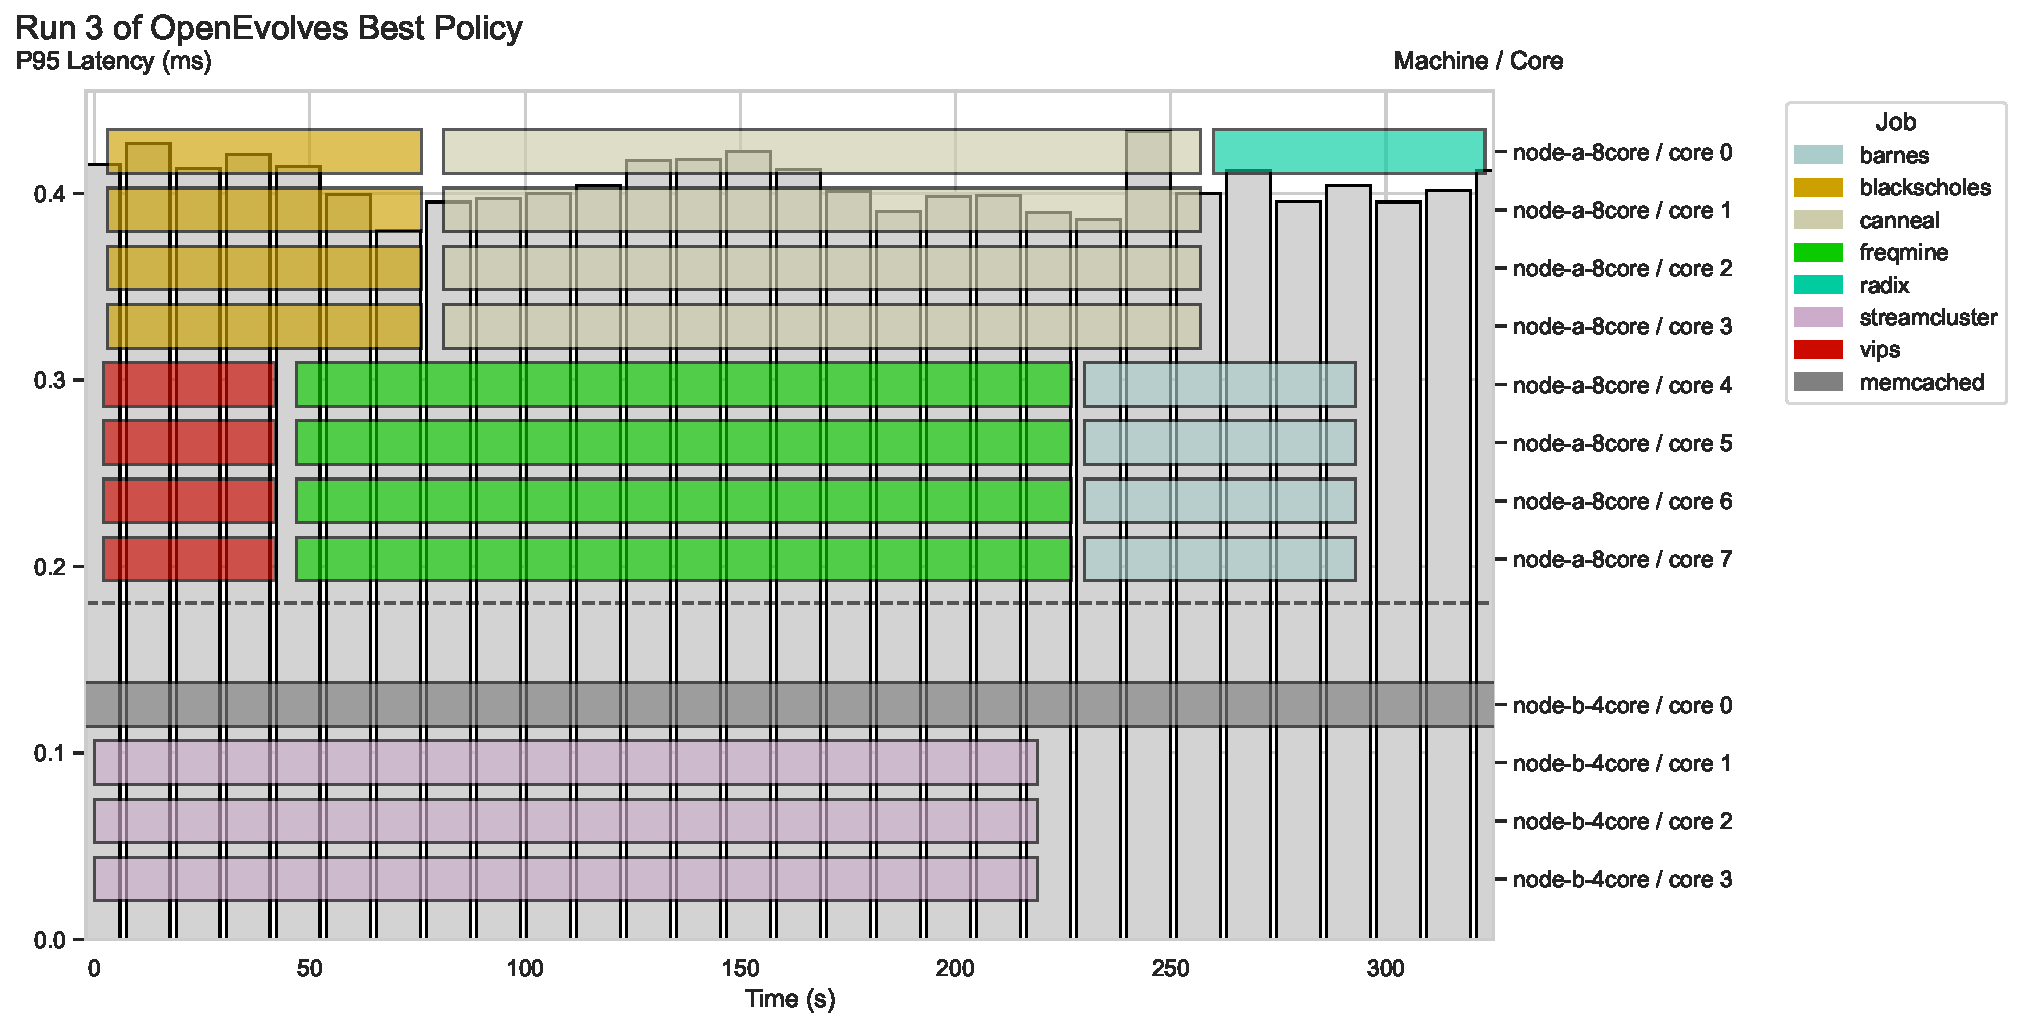
\includegraphics[width=1\linewidth]{report/figures/part3_2_2.pdf}
        \caption{Second run of the AI-generated policy. Showing the running time in seconds on the x-axis, the 95th percentile latency of memcached on the left y-axis, represented by gray vertical bars in the background), and on the right y-axis the nodes and its cores, where a color-coded vertical bar shows which job is running on that specific core. The 95th percentile latency constantly stayed below $0.5 ms$, below the given SLO. The total time to finish all jobs was $323 s$.}
        \label{fig:part3_2_2}
    \end{figure}
    
    \item Create two line plots (one for the p95 latency and one for SLO violations) showing policy performance over iterations.
    
    \textbf{Answer:}
    \end{itemize}
    \item \textbf{[17 points]} Analysis of the Evolutionary Process: Describe the process of how you used OpenEvolve to design the AI-generated policy. For example, you can include the following details in your answer (You are not limited to these questions. You can include any other details you find relevant and interesting). Your response will be graded based on the thoroughness of the exploration and clarity in explanation:
        
        \begin{itemize}
            \item How many iterations did you run through OpenEvolve with the LLMs to get to the final policy? Which LLM(s) did you use?
            \item How do you measure success? For example, how do you design the `combined\_score' or the success metric, given that there are two objectives (makespan and SLO violations)?
            \item Describe the initial policy you fed to the LLM(s) and why you chose this as the initial policy.
            \item Describe how the policy changes during the process, and how it impacted the performance of the policy (e.g., tail latency; SLO violations).
            \item Explain why did this AI-generated policy perform better (or worse) than the baseline?
            \item Identify one ``hallucination'' or logical flaw the model produced during the process and how you identified it.
        \end{itemize}

         \textbf{Answer:}
         TODO (andres): 


    \end{enumerate}

    Please attach your modified/added YAML files, run scripts, OpenEvolve scripts, experiment outputs and the report as a zip file. You can find more detailed instructions about the submission in the project description file.
    
    \textbf{Important: The search space of all possible policies is exponential and you do not have enough credits to run all of them. We do not ask you to find the policy that minimizes
    the total running time, but rather to design a policy that has a reasonable running time, does not violate the SLO, and takes into account the characteristics of the first two parts of the project.}
\end{enumerate}

\newpage
